% Intended LaTeX compiler: pdflatex
\documentclass[dvipdfmx,10pt,presentation]{beamer}
\usepackage{amsmath, amssymb, bm}
\usepackage[utf8]{inputenc}
\usepackage{indentfirst}
\usepackage[normalem]{ulem}
\usepackage{longtable}
\usepackage{minted}
\usepackage{fancyvrb}
\usetheme{Berlin}
\usepackage[utf8]{inputenc}
\usepackage[T1]{fontenc}
\usepackage{graphicx}
\usepackage{grffile}
\usepackage{longtable}
\usepackage{wrapfig}
\usepackage{rotating}
\usepackage[normalem]{ulem}
\usepackage{amsmath}
\usepackage{textcomp}
\usepackage{amssymb}
\usepackage{capt-of}
\usepackage{hyperref}
\useoutertheme[subsection=false]{smoothbars}
\setbeamertemplate{footline}[page number]
\setbeamercolor{page number in head/foot}{fg=black}
\setbeamerfont{page number in head/foot}{size=\normalsize}
\usetheme{default}
\author{情報科学類3年 江畑 拓哉 (201611350)}
\date{}
\title{自己紹介}
\begin{document}

\maketitle
\begin{frame}{Outline}
\tableofcontents
\end{frame}

\section{自己紹介}
\label{sec:org5943371}
\begin{frame}[label={sec:org6a35977}]{}
情報科学類3年知能情報メディア主専攻 江畑 拓哉\\
出身:千葉\\
好きなもの:Lisp\\
\begin{block}{最近やっていること}
\begin{center}
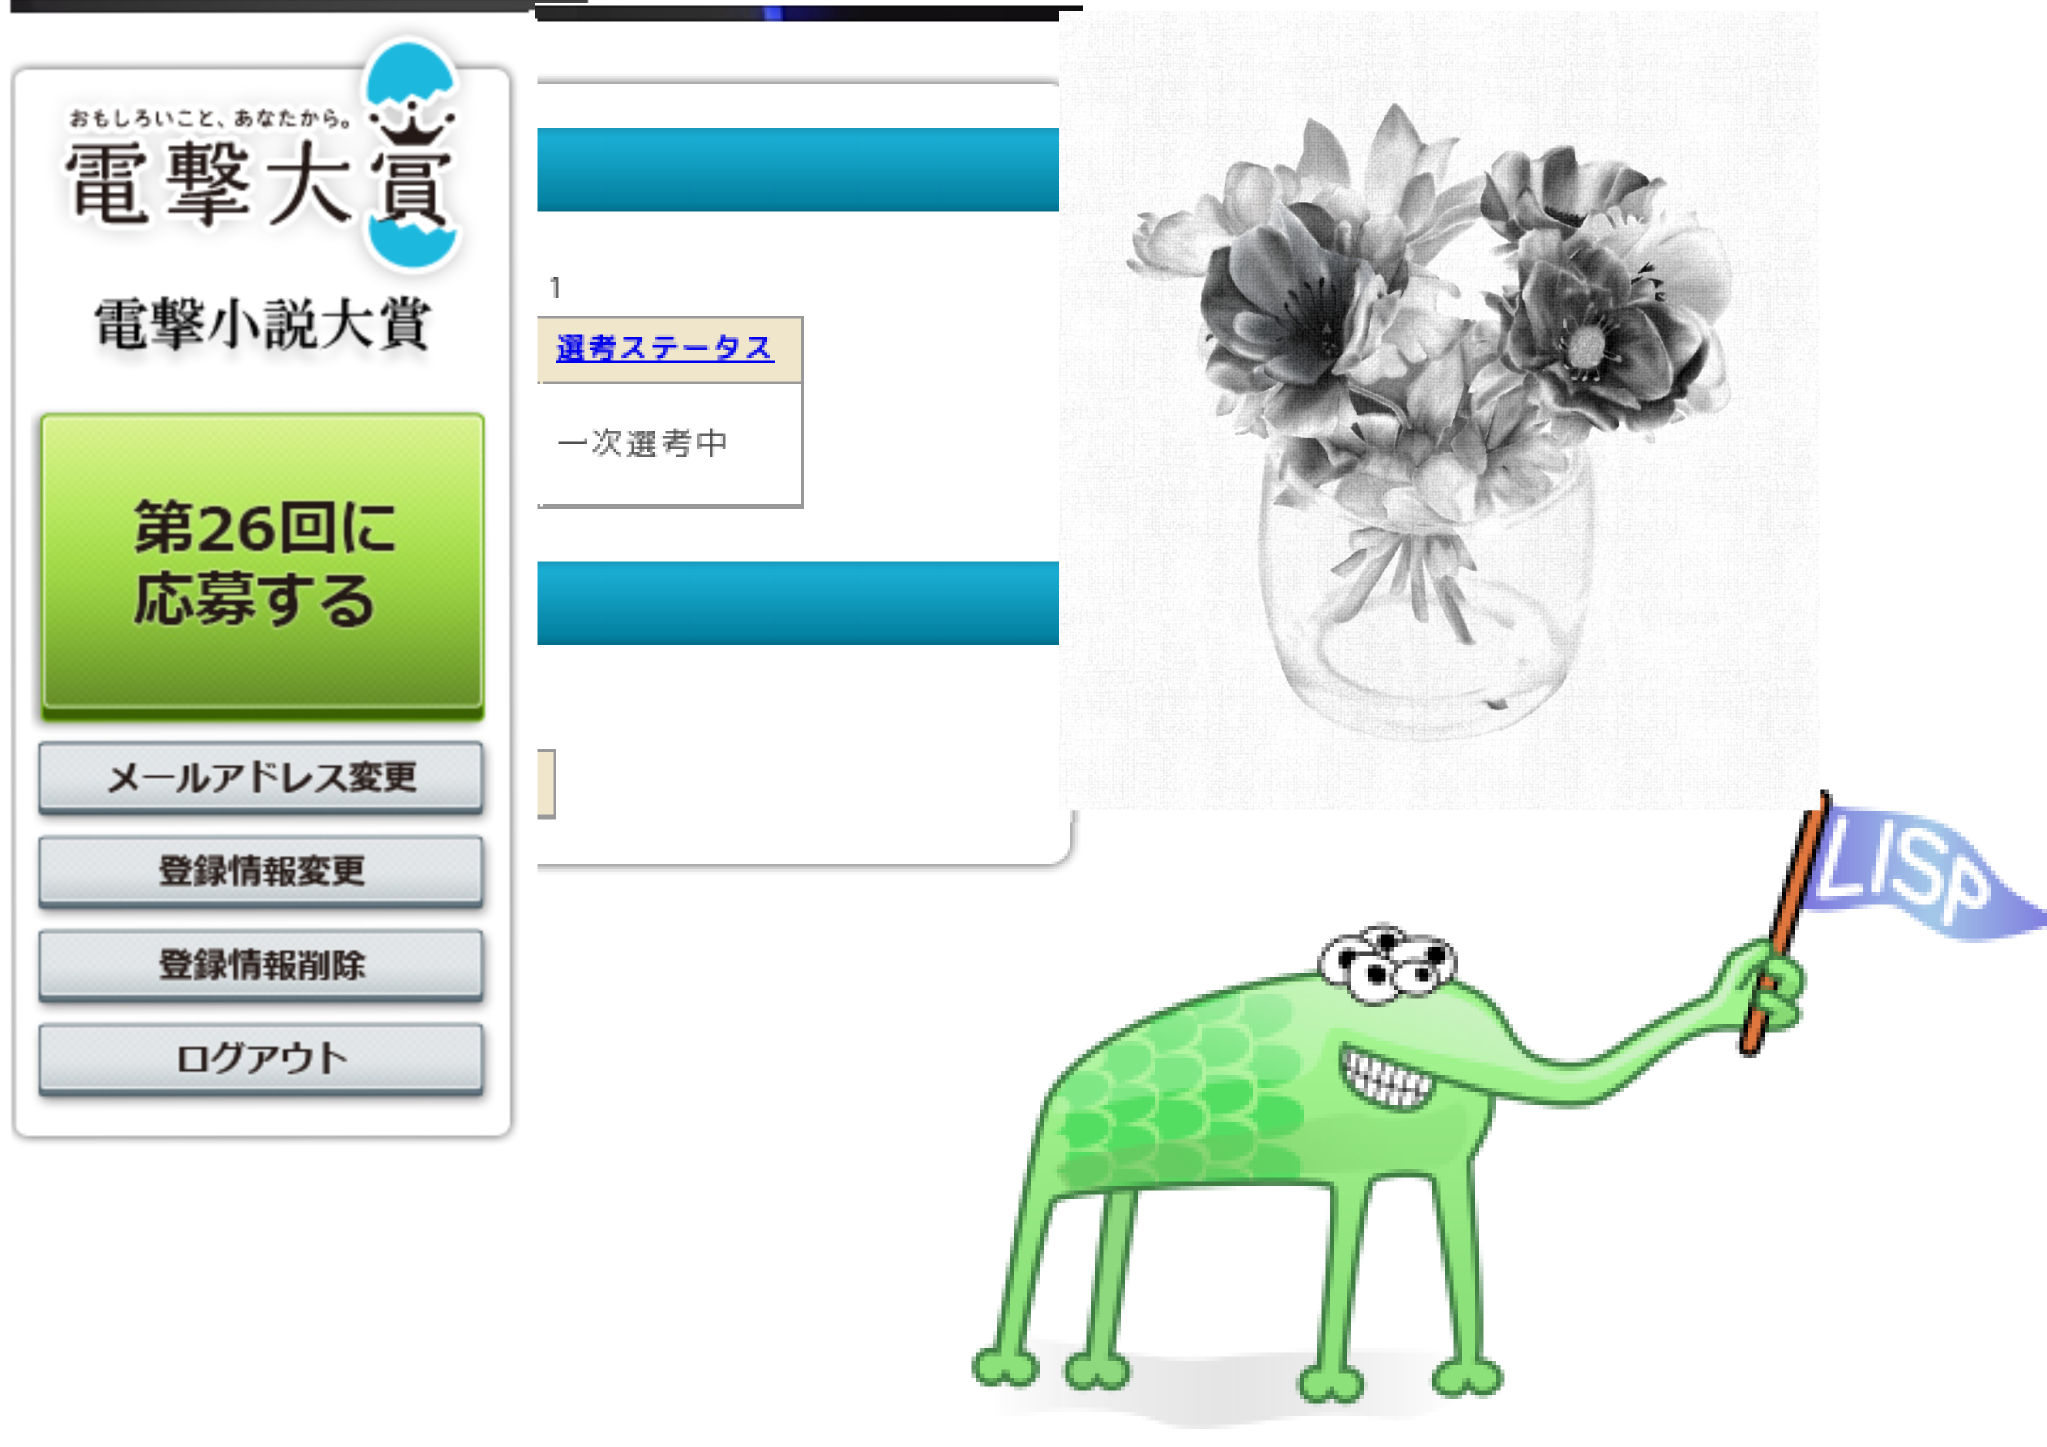
\includegraphics[width=0.7\linewidth]{./res.png}
\end{center}
\end{block}
\end{frame}
\begin{frame}[allowframebreaks]{研究テーマ}
\begin{block}{メタAI}
環境データを用いてAIを調整することで、より人との親和性を高めたい。\\
具体的には、ChatBotを作りユーザからの直接的な Q だけでなくその日の環境やユーザの体調・機嫌などによって応答を変化させてみたい。\\
\begin{itemize}
\item キーワード\\
\begin{itemize}
\item Seq2Seq(RNN LSTM) : 勉強中\\
\item Web : COJT での学習と並行して学習 (Pixijsでキャラクタを描画 websocketでサーバ内のChatBotとリアルタイム通信を行いたい)\\
\item 自然言語処理 : MeCabを使ってみたいが、先にドキュメントが豊富な英語から始めていきたいと考えている。\\
\item 他にも沢山 : どうやってユーザの情報を得るかについて(顔認識等)\\
\end{itemize}
\end{itemize}
\end{block}
\begin{block}{Web の例}
\begin{center}
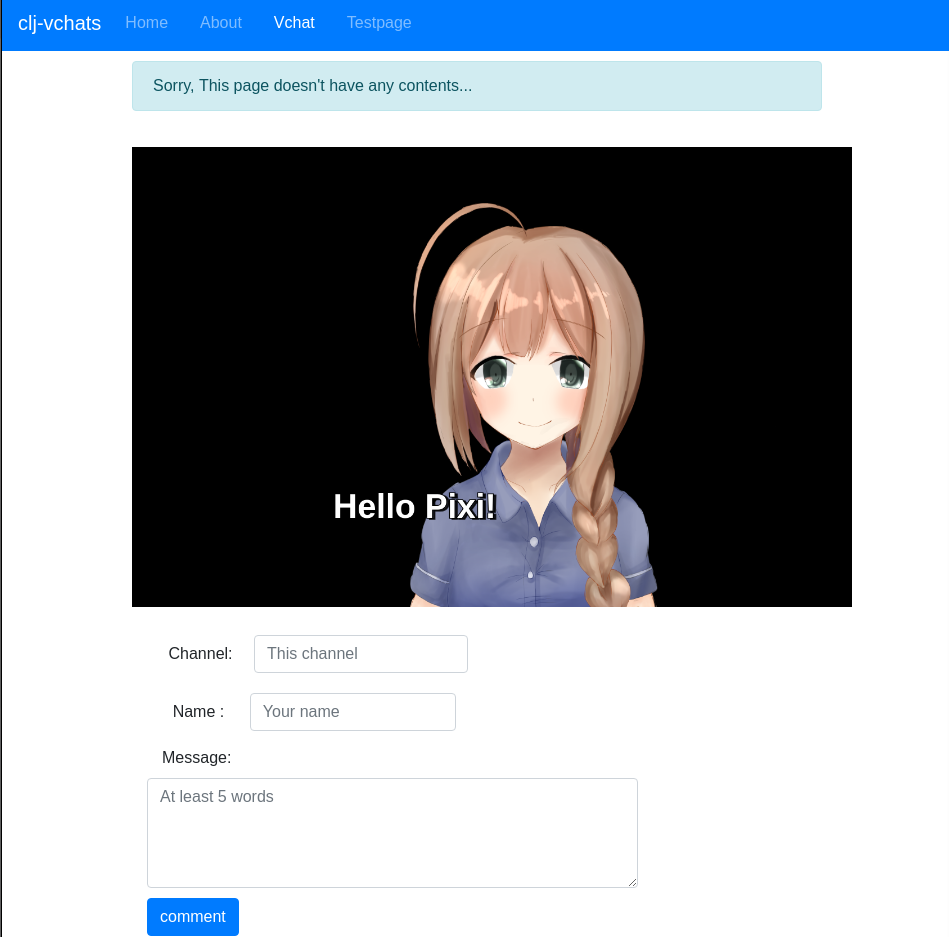
\includegraphics[width=0.7\linewidth]{./screen.png}
\end{center}
\end{block}


\begin{block}{}
\begin{center}
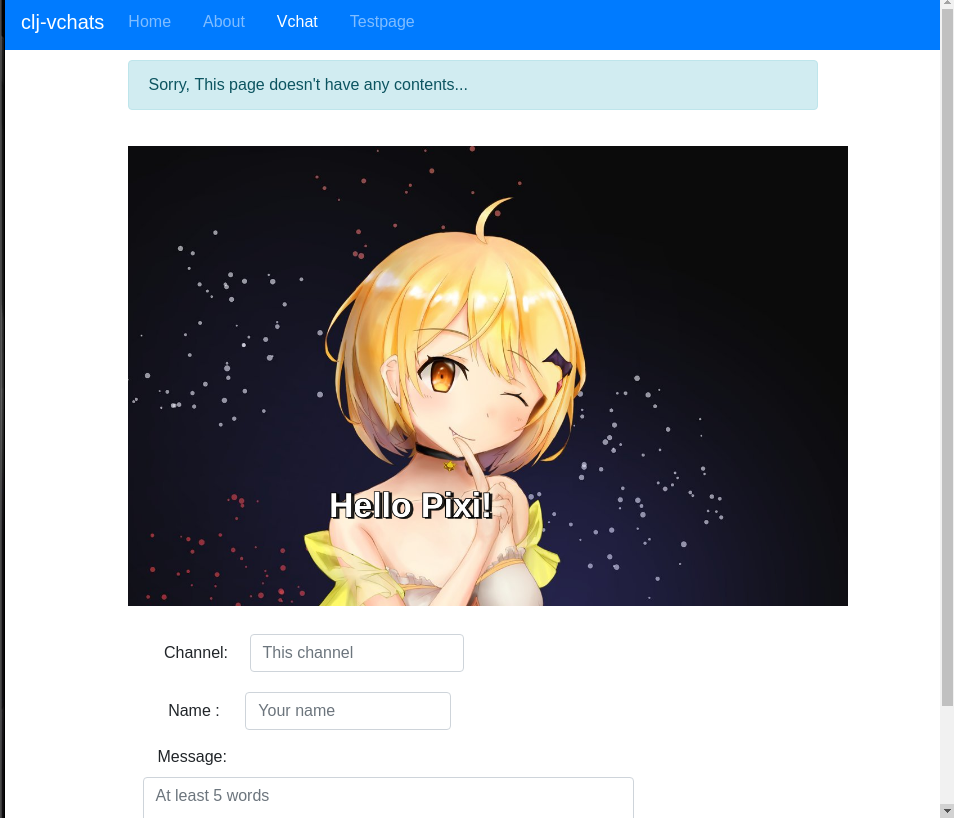
\includegraphics[width=0.7\linewidth]{./screen2.png}
\end{center}
\end{block}
\end{frame}
\end{document}
